\documentclass[11pt,a4paper]{article}

\usepackage[utf8]{inputenc}
\usepackage[T1]{fontenc}
\usepackage[spanish]{babel}
\usepackage{amsmath}
\usepackage{booktabs}
\usepackage{graphicx}
\usepackage{listings}
\usepackage{xcolor}
\usepackage[margin=2.5cm]{geometry}
\usepackage[hidelinks]{hyperref}

\addto\captionsspanish{\def\tablename{Tabla}}

% Para marcar lo que falta por completar (se ve en rojo en el PDF)
\newcommand{\pendiente}[1]{\textcolor{red}{[PENDIENTE: #1]}}
\newcommand{\pend}{\textcolor{red}{[?]}}

% Estilo para el ensamblador (los comentarios del codigo van sin tildes a proposito)
\lstdefinelanguage{riscv}{morecomment=[l]{\#}, sensitive=false}
\lstdefinestyle{asm}{
  language=riscv,
  basicstyle=\ttfamily\footnotesize,
  commentstyle=\color{gray},
  numbers=left,
  numberstyle=\tiny\color{gray},
  numbersep=6pt,
  frame=single,
  breaklines=true,
  columns=fullflexible,
  keepspaces=true,
  showstringspaces=false
}

\title{Tarea 2: M\'etricas sobre un procesador RISC-V\\[2pt]
\large Accesos a memoria, saltos y operaciones entre registros en un pipeline de 5 etapas}
\author{Jorge Pablo Porras Alvarado \\ Josué Adrián Pérez Pérez \\ \pendiente{nombres de los dem\'as integrantes del grupo}}
\date{\today}

\begin{document}

\maketitle

\begin{center}
Instituto Tecnol\'ogico de Costa Rica \\
Escuela de Ingenier\'ia en Computadores \\
CE 1107 --- Fundamentos de Arquitectura de Computadores \\
Profesor: Luis Chavarr\'ia Zamora
\end{center}

\vspace{1em}

%==========================================================
\section{Introducci\'on}
%==========================================================

El desempe\~no de un procesador con pipeline depende del tipo de instrucciones
que ejecuta y de c\'omo resuelve las dependencias entre ellas. Esta tarea mide,
con el simulador Ripes~\cite{ripes}, tres aspectos del funcionamiento de un
procesador RISC-V: la cantidad de accesos a memoria, los saltos y las
operaciones entre registros. Para cada aspecto se dise\~na un programa en
ensamblador que realiza miles de operaciones de ese tipo, se cuantifican de
forma anal\'itica y se comprueban con la informaci\'on de ejecuci\'on
(\emph{Execution info}) del simulador.

Cada programa se ejecuta en dos procesadores de 5 etapas de Ripes:

\begin{enumerate}
  \item un pipeline \textbf{con} unidad de forwarding y detecci\'on de hazards, y
  \item un pipeline \textbf{sin} ninguno de los dos, donde los riesgos se
        resuelven por software mediante transformaci\'on de c\'odigo.
\end{enumerate}

El documento presenta primero el marco te\'orico, luego el desarrollo de cada
programa, despu\'es la discusi\'on de los resultados y, finalmente, las
conclusiones. \pendiente{revisar esta introducci\'on cuando est\'en las tres partes}

%==========================================================
\section{Marco te\'orico}
%==========================================================

\paragraph{Accesos a memoria.}
En un procesador con pipeline de cinco etapas (IF, ID, EX, MEM, WB), cada
instrucci\'on lee la memoria de instrucciones en la etapa IF, y solo las
cargas y los almacenamientos acceden a la memoria de datos, en la etapa MEM
\cite{harris,patterson}. Por lo tanto, el n\'umero de accesos a la memoria de
datos de un programa es igual al n\'umero de \texttt{lw}/\texttt{sw}
ejecutados, y el de accesos a la memoria de instrucciones es al menos el
n\'umero de instrucciones retiradas.

\paragraph{Rendimiento.}
El tiempo de ejecuci\'on de un programa se descompone como
\begin{equation}
  T = N_{\text{instr}} \times \text{CPI} \times T_c ,
\end{equation}
donde $N_{\text{instr}}$ es el n\'umero de instrucciones, CPI los ciclos por
instrucci\'on y $T_c$ el periodo del reloj \cite{harris,patterson}. En un
pipeline ideal el CPI tiende a 1, y cada atasco o burbuja lo aumenta.

\paragraph{Hazards de datos.}
Una instrucci\'on escribe su resultado en el banco de registros en la etapa WB
(etapa 5), pero la instrucci\'on siguiente lee sus operandos en ID (etapa 2).
Si la que lee es una instrucci\'on cercana a la que escribe (dependencia
\emph{read after write}, RAW), puede leer el valor viejo. Las dependencias
WAR y WAW no causan problemas en este pipeline, porque las instrucciones
avanzan en orden. El forwarding resuelve las RAW enviando el resultado
directamente a la ALU sin esperar a WB. Si no existe ese hardware, hay que dejar
una distancia suficiente entre las dos instrucciones, insertando \texttt{nop}
(\texttt{addi zero, zero, 0}) o reordenando c\'odigo. En el modelo de Ripes
utilizado, esa distancia m\'inima result\'o ser de 3 instrucciones, es decir,
2 \texttt{nop} entre dos instrucciones dependientes consecutivas (se verifica
experimentalmente en la secci\'on~\ref{sec:parte1}).

\paragraph{Hazards de control.}
Un salto tomado no se resuelve hasta la etapa EX, de modo que para entonces ya
se buscaron instrucciones de m\'as que deben descartarse. Eso introduce una
penalizaci\'on de ciclos por cada salto tomado, que el forwarding no elimina.
En los resultados de la secci\'on~\ref{sec:resultados} se observa una
penalizaci\'on de 2 ciclos por salto tomado.

\paragraph{Saltos.}
RISC-V tiene dos tipos de instrucciones que cambian el flujo del programa: los
saltos \emph{condicionales} (\texttt{beq}, \texttt{bne}, \texttt{blt},
\texttt{bge}, etc.), que saltan solo si se cumple una comparaci\'on entre dos
registros, y los saltos \emph{incondicionales} (\texttt{jal}, \texttt{jalr}),
que siempre saltan \cite{harris,patterson}. Un salto condicional puede ser
\emph{tomado} o \emph{no tomado}; uno incondicional siempre es tomado.
 
Mientras un salto se resuelve en EX, el procesador sigue buscando las
instrucciones que vienen despu\'es en memoria, es decir, se comporta como si
predijera que el salto \emph{no} se toma. Si el salto no se toma, esas
instrucciones son las correctas y no se pierde ning\'un ciclo; si se toma, hay
que descartarlas. Por lo tanto, la penalizaci\'on depende solo de los saltos
tomados \cite{patterson}. Las t\'ecnicas de predicci\'on de saltos buscan
reducir esa penalizaci\'on adivinando el resultado antes de EX, a partir del
sentido del salto o de su historial de ejecuci\'on \cite{smith}.

\pendiente{agregar el marco te\'orico de operaciones
entre registros (Parte 3), con referencias IEEE}

%==========================================================
\section{Desarrollo}
%==========================================================

%----------------------------------------------------------
\subsection{Parte 1: Accesos a memoria}
\label{sec:parte1}
%----------------------------------------------------------

\subsubsection{Programa}

El programa recorre un arreglo de $N=2000$ palabras y guarda en cada posici\'on
el valor de su propio \'indice. Para forzar tanto escrituras como lecturas,
despu\'es de cada \texttt{sw} se hace un \texttt{lw} de la misma posici\'on. El
c\'odigo final, con la cuantificaci\'on de accesos en los comentarios, es:

\begin{lstlisting}[style=asm,caption={Programa de accesos a memoria (versi\'on para el procesador con hazard unit).},label={lst:original}]
    addi s2, zero, 0      # idx: i = 0
    addi t2, zero, 2000   # N = 2000
    lui  s1, 0x10000      # base = 0x10000000 (inicio del segmento de datos)
    lui  t0, 0x00000      # no se usa, slli lo sobrescribe (se deja tal como se corrio)

FOR:
    bge  s2, t2, done     # salta si i >= N: 2001 evaluaciones, solo la ultima salta
    slli t0, s2, 2        # t0 = 4*i (operacion entre registros)
    add  t0, t0, s1       # t0 = base + 4*i (operacion entre registros)
    sw   s2, 0(t0)        # ESCRITURA a memoria de datos: 1 por vuelta x 2000 = 2000
    lw   s3, 0(t0)        # LECTURA de memoria de datos: 1 por vuelta x 2000 = 2000
    addi s2, s2, 1        # i = i + 1
    jal  zero, FOR        # salto incondicional: 2000 veces

done:
    li   a0, 10           # syscall exit
    ecall                 # accesos totales a memoria de datos = 2000 + 2000 = 4000
\end{lstlisting}

\paragraph{Cuantificaci\'on.}
Cada vuelta ejecuta 7 instrucciones. Con las 4 de inicio y las 3 del final (el
\texttt{bge} que sale del ciclo, \texttt{li} y \texttt{ecall}):
\begin{align}
  N_{\text{instr}} &= 4 + 7 \times 2000 + 3 = 14007, \\
  N_{\text{datos}} &= \underbrace{2000}_{\texttt{sw}} + \underbrace{2000}_{\texttt{lw}} = 4000 .
\end{align}
Adem\'as, cada instrucci\'on retirada implica al menos una lectura de la
memoria de instrucciones, as\'i que hay al menos 14007 lecturas de instrucci\'on
contra 4000 accesos a datos.

\paragraph{Por qu\'e funciona.}
Cada palabra ocupa 4 bytes, de modo que la direcci\'on del elemento $i$ es
\begin{equation}
  \text{dir}(i) = \text{base} + 4i .
\end{equation}
El desplazamiento a la izquierda $i \ll 2$ equivale a multiplicar por 4, que es
lo que hace \texttt{slli t0, s2, 2}. La base $\texttt{0x10000000}$ y los
desplazamientos son m\'ultiplos de 4, por lo que todos los accesos de palabra
est\'an alineados. La condici\'on \texttt{bge s2, t2, done} se eval\'ua al
inicio de cada vuelta, as\'i que el cuerpo se ejecuta exactamente mientras
$i < 2000$, es decir, 2000 veces, y la condici\'on se eval\'ua 2001 veces.

\paragraph{Verificaci\'on.}
Al terminar, la memoria debe contener $0, 1, \dots, 1999$ en palabras
consecutivas a partir de $\texttt{0x10000000}$. El \'ultimo elemento est\'a en
\begin{equation}
  \texttt{0x10000000} + 4 \times 1999 = \texttt{0x10001F3C},
\end{equation}
y la direcci\'on $\texttt{0x10001F40}$, que ser\'ia el elemento 2000, debe
seguir en cero porque el ciclo se detuvo antes de escribirla.

\begin{figure}[h]
  \centering
  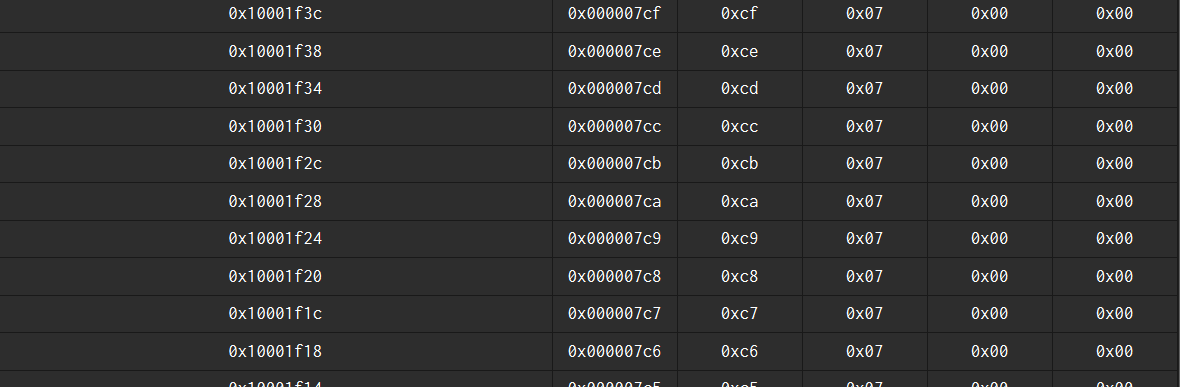
\includegraphics[width=0.9\textwidth]{captura_memoria.png}
  \caption{Pesta\~na Memory de Ripes tras la ejecuci\'on: el \'ultimo elemento,
  $\texttt{0x000007CF} = 1999$, est\'a en $\texttt{0x10001F3C}$, y las
  palabras anteriores decrecen de uno en uno.}
\end{figure}



\subsubsection{Versi\'on para el procesador sin hardware de riesgos}

En el modelo sin forwarding ni detecci\'on de hazards, las dependencias RAW
entre instrucciones cercanas producir\'ian resultados incorrectos. La
soluci\'on es la transformaci\'on de c\'odigo: insertar \texttt{nop} hasta que
la instrucci\'on que lee quede a una distancia de al menos 3 instrucciones de
la que escribe. La Tabla~\ref{tab:dependencias} resume los pares RAW del
programa.

\begin{table}[h]
  \centering
  \small
  \begin{tabular}{@{}llcccc@{}}
    \toprule
    Escribe & Lee & Reg. & Dist. original & \texttt{nop} & Dist. final \\
    \midrule
    \texttt{slli t0}      & \texttt{add t0}        & \texttt{t0} & 1 & 2 & 3 \\
    \texttt{add t0}       & \texttt{sw 0(t0)}      & \texttt{t0} & 1 & 2 & 3 \\
    \texttt{add t0}       & \texttt{lw 0(t0)}      & \texttt{t0} & 2 & (los mismos 2) & 4 \\
    \texttt{addi s2}      & \texttt{bge} (sig. vuelta) & \texttt{s2} & 2 & 2 & 4 \\
    \texttt{addi s2}      & \texttt{slli} (sig. vuelta) & \texttt{s2} & 3 & 0 & 5 \\
    \texttt{addi t2} (inicio) & primer \texttt{bge} & \texttt{t2} & 3 & 0 & 3 \\
    \texttt{addi s2} (inicio) & primer \texttt{bge} & \texttt{s2} & 4 & 0 & 4 \\
    \bottomrule
  \end{tabular}
  \caption{Dependencias RAW y \texttt{nop} colocados. La distancia es el n\'umero de
  posiciones entre las dos instrucciones en el orden del programa.}
  \label{tab:dependencias}
\end{table}

Algunas observaciones sobre la tabla:
\begin{itemize}
  \item El \texttt{sw} y el \texttt{lw} de la misma direcci\'on no generan un
        hazard de registros, porque las dos instrucciones acceden a memoria en
        orden.
  \item Los dos \texttt{nop} antes del \texttt{jal} se colocaron para garantizar
        la distancia m\'inima entre \texttt{addi s2} y el \texttt{bge} de la
        vuelta siguiente en el orden del programa, sin depender de los ciclos
        de burbuja que introduce el salto.
  \item Los pares de inicio con distancia 3 y 4 funcionaron sin \texttt{nop}:
        el primer \texttt{bge} lee \texttt{t2} a distancia 3 y el programa
        llen\'o la memoria correctamente. Si hubiera le\'ido el valor
        anterior (cero), habr\'ia comparado $0 \ge 0$ y habr\'ia salido sin
        escribir nada. Esto confirma que la distancia 3 es suficiente en este
        modelo.
  \item Tras el \texttt{jal} no se colocaron \texttt{nop}. El comportamiento
        observado es consistente con que el procesador descarta las
        instrucciones buscadas despu\'es de un salto tomado
        (secci\'on~\ref{sec:resultados}).
  \item El registro \texttt{s3} cargado por \texttt{lw} no se utiliza despu\'es,
        por lo que este programa no presenta el hazard de carga seguida de
        uso.
\end{itemize}

El c\'odigo transformado es:

\begin{lstlisting}[style=asm,caption={Versi\'on con \texttt{nop} para el procesador sin forwarding ni detecci\'on de hazards.},label={lst:nops}]
    addi s2, zero, 0      # idx: i = 0
    addi t2, zero, 2000   # N = 2000
    lui  s1, 0x10000      # base = 0x10000000
    lui  t0, 0x00000      # no se usa

FOR:
    bge  s2, t2, done     # salta si i >= N
    slli t0, s2, 2        # t0 = 4*i
    nop                   # RAW slli -> add: se necesitan 2 nop
    nop
    add  t0, t0, s1       # t0 = base + 4*i
    nop                   # RAW add -> sw y add -> lw: se necesitan 2 nop
    nop
    sw   s2, 0(t0)        # ESCRITURA: 2000 en total
    lw   s3, 0(t0)        # LECTURA: 2000 en total
    addi s2, s2, 1        # i = i + 1
    nop                   # distancia minima hasta el bge de la vuelta siguiente
    nop
    jal  zero, FOR        # salto incondicional

done:
    li   a0, 10
    ecall
\end{lstlisting}

Esta versi\'on ejecuta 13 instrucciones por vuelta (7 \'utiles y 6
\texttt{nop}), por lo que
\begin{equation}
  N_{\text{instr}} = 4 + 13 \times 2000 + 3 = 26007 .
\end{equation}
Los \texttt{nop} no tocan la memoria de datos, as\'i que los accesos a datos
siguen siendo 4000.

\subsubsection{Resultados}
\label{sec:resultados}

La Tabla~\ref{tab:resultados} reporta la informaci\'on de ejecuci\'on (Execution
info) de Ripes para cada procesador.

\begin{table}[h]
  \centering
  \begin{tabular}{@{}lrr@{}}
    \toprule
    M\'etrica & Sin hazard (con \texttt{nop}) & Con hazard (original) \\
    \midrule
    Ciclos                          & 30013  & 18013  \\
    Instrucciones retiradas         & 26007  & 14007  \\
    CPI                             & 1.15   & 1.29   \\
    IPC                             & 0.867  & 0.778  \\
    \texttt{nop} ejecutados         & 12000  & 0      \\
    Accesos a memoria de datos      & 4000   & 4000   \\
    Saltos tomados                  & 2001   & 2001   \\
    \bottomrule
  \end{tabular}
  \caption{M\'etricas obtenidas en Ripes para el programa de accesos a memoria en ambos procesadores.}
  \label{tab:resultados}
\end{table}

\begin{figure}[h]
  \centering
  \begin{minipage}[t]{0.42\textwidth}
    \centering
    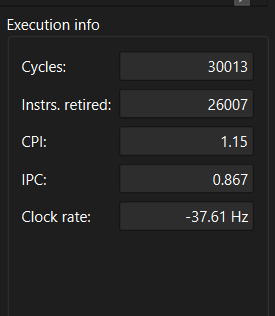
\includegraphics[width=\textwidth]{execinfo_sin_hazard.png}\\[2pt]
    {\small (a) Sin hazard (con \texttt{nop})}
  \end{minipage}\hfill
  \begin{minipage}[t]{0.42\textwidth}
    \centering
    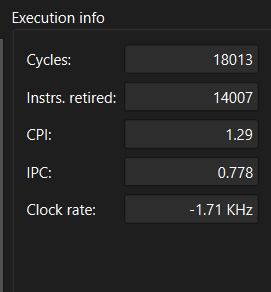
\includegraphics[width=\textwidth]{execinfo_con_hazard.png}\\[2pt]
    {\small (b) Con hazard (original)}
  \end{minipage}
  \caption{Execution info de Ripes en cada procesador. El campo Clock rate no
  se utiliza en el an\'alisis.}
\end{figure}

\paragraph{Modelo de ciclos.}
En ambos procesadores los ciclos se ajustan exactamente a
\begin{equation}
  C = N_{\text{instr}} + 4 + 2\,N_{\text{saltos}} ,
\end{equation}
donde 4 ciclos son el llenado del pipeline y $N_{\text{saltos}}$ cuenta los
saltos tomados. Con 2001 saltos tomados (los 2000 \texttt{jal} m\'as el
\texttt{bge} final):
\begin{align}
  \text{con hazard:} &\quad 14007 + 4 + 2 \times 2001 = 18013, \\
  \text{sin hazard:} &\quad 26007 + 4 + 2 \times 2001 = 30013 .
\end{align}
Esto es consistente con una penalizaci\'on de 2 ciclos por salto tomado, la que
corresponde a descartar las 2 instrucciones buscadas antes de que el salto se
resuelva en EX. 

%----------------------------------------------------------
\subsection{Parte 2: Saltos}
%----------------------------------------------------------

\label{sec:parte2}
 
\subsubsection{Programa}
 
Para comprobar que solo los saltos tomados tienen costo, el programa debe
ejecutar saltos tomados y no tomados en cantidades conocidas. Se recorre un
ciclo de $N=2000$ vueltas y, en cada una, un salto condicional decide si el
\'indice $i$ es par o impar: si es par, salta a sumar un contador de pares; si
es impar, no salta, suma un contador de impares y luego salta
incondicionalmente al final del cuerpo. La condici\'on del ciclo se eval\'ua al
final de cada vuelta. El c\'odigo final es:
 
\begin{lstlisting}[style=asm,caption={Programa de saltos (versi\'on para el procesador con hazard unit).},label={lst:saltos}]
    addi s2, zero, 0 #idx: i = 0
    addi t2, zero, 2000 #N = 2000
    addi s1, zero, 0 # contador impares
    addi s0, zero, 0 # contador pares
LOOP:
    andi t0, s2, 1 # se ejecuta 2000 veces
    beq t0, zero, PAR # se ejecuta 2000 veces, se toma el salto 1000 veces y no se toma 1000 veces
    addi s1, s1, 1 # suma impares, se ejecuta 1000 veces
    jal zero, SIGUE # se toma este salto 1000 veces
PAR:
    addi s0, s0, 1 # suma pares, se ejecuta 1000 veces
SIGUE:
    addi s2, s2, 1 # se ejecuta 2000 veces
    blt s2, t2, LOOP # se toma el salto 1999 veces y no se toma 1 vez
done:
    li a7, 10 # syscall exit
    nop
    nop
    nop
    ecall
# se ejecutan 5000 saltos, de los cuales solo se toman 3999 y no se toman 1001
\end{lstlisting}
 
Los tres \texttt{nop} antes del \texttt{ecall} no forman parte de la medici\'on
de saltos; su justificaci\'on se da en la secci\'on~\ref{sec:ecall}.
 
\paragraph{Cuantificaci\'on.}
La Tabla~\ref{tab:saltos} resume cu\'antas veces se ejecuta cada salto y cu\'antas
veces se toma.
 
\begin{table}[h]
  \centering
  \begin{tabular}{@{}lrrr@{}}
    \toprule
    Instrucci\'on & Ejecuciones & Tomados & No tomados \\
    \midrule
    \texttt{beq t0, zero, PAR}  & 2000 & 1000 & 1000 \\
    \texttt{jal zero, SIGUE}    & 1000 & 1000 & 0    \\
    \texttt{blt s2, t2, LOOP}   & 2000 & 1999 & 1    \\
    \midrule
    Total                       & 5000 & 3999 & 1001 \\
    \bottomrule
  \end{tabular}
  \caption{Cuantificaci\'on de los saltos del programa.}
  \label{tab:saltos}
\end{table}
 
Las vueltas pares ejecutan 5 instrucciones (\texttt{andi}, \texttt{beq},
\texttt{addi s0}, \texttt{addi s2}, \texttt{blt}) y las impares 6, porque se
agregan \texttt{addi s1} y \texttt{jal}. Con las 4 instrucciones de inicio y
las 5 del final (\texttt{li}, tres \texttt{nop} y \texttt{ecall}):
\begin{align}
  N_{\text{instr}} &= 4 + 1000 \times 5 + 1000 \times 6 + 5 = 11009, \\
  N_{\text{tomados}} &= 1000 + 1000 + 1999 = 3999 .
\end{align}
 
\paragraph{Por qu\'e funciona.}
La instrucci\'on \texttt{andi t0, s2, 1} conserva solo el bit menos
significativo de $i$, que vale 0 si $i$ es par y 1 si es impar. Como $i$
recorre los valores $0, 1, \dots, 1999$, hay exactamente 1000 pares y 1000
impares, de modo que el \texttt{beq} se toma 1000 veces y no se toma otras
1000. El \texttt{jal} solo se ejecuta en el camino impar, as\'i que se ejecuta
1000 veces y siempre se toma. Como la condici\'on del ciclo est\'a al final, el
cuerpo se ejecuta para $i = 0$ antes de evaluar \texttt{blt}; despu\'es de
incrementar, \texttt{blt} compara $i+1 < 2000$, que se cumple 1999 veces y
falla una sola vez, cuando $i+1 = 2000$.
 
\paragraph{Verificaci\'on.}
Al terminar, los contadores deben valer $\texttt{s0} = \texttt{s1} = 1000 =
\texttt{0x3E8}$, lo que demuestra que cada camino del \texttt{beq} se ejecut\'o
las veces calculadas.
 
\begin{figure}[h]
  \centering
  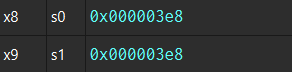
\includegraphics[width=0.9\textwidth]{memoria2.png}
  \caption{Estado de los registros $\texttt{s0}$ y $\texttt{s1}$ al concluir el programa,}
\end{figure}
 
\subsubsection{Versi\'on para el procesador sin hardware de riesgos}
 
Los saltos tambi\'en leen registros, por lo que participan en dependencias RAW.
La Tabla~\ref{tab:dependencias2} resume los pares del programa y los
\texttt{nop} insertados con la misma regla de la Parte~1: una distancia m\'inima
de 3 instrucciones entre la que escribe y la que lee.
 
\begin{table}[h]
  \centering
  \small
  \begin{tabular}{@{}llcccc@{}}
    \toprule
    Escribe & Lee & Reg. & Dist. original & \texttt{nop} & Dist. final \\
    \midrule
    \texttt{andi t0}          & \texttt{beq t0}                & \texttt{t0} & 1 & 2 & 3 \\
    \texttt{addi s2} (SIGUE)  & \texttt{blt s2}                & \texttt{s2} & 1 & 2 & 3 \\
    \texttt{addi s2} (SIGUE)  & \texttt{andi} (sig. vuelta)    & \texttt{s2} & 2 & (los mismos 2) & 4 \\
    \texttt{addi s2} (inicio) & primer \texttt{andi}           & \texttt{s2} & 4 & 0 & 4 \\
    \texttt{addi s0} (inicio) & primer \texttt{addi s0}        & \texttt{s0} & 5 & 0 & 5 \\
    \texttt{li a7}            & \texttt{ecall}                 & \texttt{a7} & 1 & 3 & 4 \\
    \bottomrule
  \end{tabular}
  \caption{Dependencias RAW del programa de saltos y \texttt{nop} colocados. La
  distancia se mide en el orden de ejecuci\'on.}
  \label{tab:dependencias2}
\end{table}
 
Los contadores \texttt{s0} y \texttt{s1} solo se vuelven a leer en vueltas
posteriores, muy lejos de su escritura. Despu\'es de los saltos tomados no se
colocaron \texttt{nop}, porque el procesador descarta las instrucciones buscadas
en el camino equivocado (secci\'on~\ref{sec:resultados}). El c\'odigo
transformado es:
 
\begin{lstlisting}[style=asm,caption={Versi\'on con \texttt{nop} para el procesador sin forwarding ni detecci\'on de hazards.},label={lst:saltos_nops}]
    addi s2, zero, 0 #idx: i = 0
    addi t2, zero, 2000 #N = 2000
    addi s1, zero, 0 # contador impares
    addi s0, zero, 0 # contador pares
LOOP:
    andi t0, s2, 1 # se ejecuta 2000 veces
    nop # RAW andi -> beq (t0): 2 nop
    nop
    beq t0, zero, PAR # se ejecuta 2000 veces, se toma el salto 1000 veces y no se toma 1000 veces
    addi s1, s1, 1 # suma impares, se ejecuta 1000 veces
    jal zero, SIGUE # se toma este salto 1000 veces
PAR:
    addi s0, s0, 1 # suma pares, se ejecuta 1000 veces
SIGUE:
    addi s2, s2, 1 # se ejecuta 2000 veces
    nop # RAW addi -> blt (s2): 2 nop
    nop
    blt s2, t2, LOOP # se toma el salto 1999 veces y no se toma 1 vez, se ejecuta 2000 veces
done:
    li a7, 10 # syscall exit
    nop
    nop
    nop
    ecall
# se ejecutan 5000 saltos, de los cuales solo se toman 3999 y no se toman 1001
\end{lstlisting}
 
Se agregan 4 \texttt{nop} por vuelta, as\'i que
\begin{equation}
  N_{\text{instr}} = 11009 + 4 \times 2000 = 19009 .
\end{equation}
Los \texttt{nop} no son saltos, por lo que la cuantificaci\'on de la
Tabla~\ref{tab:saltos} no cambia.
 
\subsubsection{Terminaci\'on del programa: el \texttt{ecall}}
\label{sec:ecall}
 
En Ripes, el n\'umero de llamada al sistema se pasa en \texttt{a7}; con
$\texttt{a7} = 10$, \texttt{ecall} termina el programa. Al probar distintas
formas de terminar se encontr\'o que el \texttt{ecall} tiene un costo y un
comportamiento propios, resumidos en la Tabla~\ref{tab:ecall}.
 
\begin{table}[h]
  \centering
  \small
  \begin{tabular}{@{}lllc@{}}
    \toprule
    Procesador & Antes del \texttt{ecall} & Resultado & Ciclos extra \\
    \midrule
    Con hazard unit & \texttt{li a7} a distancia 1           & termina bien & 2 \\
    Con hazard unit & \texttt{li a7} + 3 \texttt{nop}        & termina bien & 2 \\
    Con hazard unit & \texttt{blt} (\texttt{li a7} al inicio) & termina bien & 1 \\
    Sin hazard unit & \texttt{li a7} + 3 \texttt{nop}        & termina bien & 0 \\
    Sin hazard unit & \texttt{blt} (\texttt{li a7} al inicio) & termina tras 1 vuelta & --- \\
    \bottomrule
  \end{tabular}
  \caption{Comportamiento del \texttt{ecall} de salida seg\'un el procesador y
  lo que lo precede. Los ciclos extra son los que exceden el modelo de la
  ecuaci\'on~\eqref{eq:modelo2}.}
  \label{tab:ecall}
\end{table}
 
El c\'odigo fuente de Ripes explica estos resultados \cite{ripes_src}:
 
\begin{itemize}
  \item \textbf{Con hazard unit}, el \texttt{ecall} se atiende en la etapa EX.
        Como depende impl\'icitamente de todos los registros, la unidad de
        hazards lo detiene mientras alguna instrucci\'on en MEM o WB tenga una
        escritura pendiente al banco de registros. Si las dos instrucciones
        anteriores escriben un registro, el atasco es de 2 ciclos; si solo la
        segunda anterior escribe (el \texttt{blt} no escribe), es de 1 ciclo.
        Los \texttt{nop} (\texttt{addi zero, zero, 0}) cuentan como escrituras,
        por lo que no evitan el atasco.
  \item \textbf{Sin hazard unit}, el \texttt{ecall} se atiende en la etapa ID,
        sin ning\'un atasco. Por eso necesita que \texttt{li a7} est\'e a
        distancia 4 (tres \texttt{nop}). Adem\'as, si el \texttt{ecall} est\'a
        justo despu\'es del \texttt{blt}, llega a ID en el mismo ciclo en que el
        \texttt{blt} se resuelve en EX y se ejecuta antes de ser descartado.
        Con \texttt{a7} ya cargado desde el inicio, el programa termin\'o al
        final de la primera vuelta, con $\texttt{s0} = 1$ y $\texttt{s1} = 0$.
\end{itemize}
 
El \'ultimo caso es un hazard de control sobre una instrucci\'on con efectos
fuera del pipeline: una instrucci\'on buscada en el camino equivocado de un
salto no deber\'ia tener efectos hasta que el salto se confirme. Por estas
razones, ambas versiones finales terminan con \texttt{li a7, 10} seguido de
tres \texttt{nop} antes del \texttt{ecall}.
 
\subsubsection{Resultados}
\label{sec:resultados2}
 
\begin{table}[h]
  \centering
  \begin{tabular}{@{}lrr@{}}
    \toprule
    M\'etrica & Sin hazard (con \texttt{nop}) & Con hazard (original) \\
    \midrule
    Ciclos                          & 27011  & 19013  \\
    Instrucciones retiradas         & 19009  & 11009  \\
    CPI                             & 1.42   & 1.73   \\
    IPC                             & 0.704  & 0.579  \\
    \texttt{nop} ejecutados         & 8003   & 3      \\
    Saltos ejecutados               & 5000   & 5000   \\
    Saltos tomados / no tomados     & 3999 / 1001 & 3999 / 1001 \\
    \bottomrule
  \end{tabular}
  \caption{M\'etricas obtenidas en Ripes para el programa de saltos en ambos procesadores.}
  \label{tab:resultados2}
\end{table}
 
\begin{figure}[h]
  \centering
  \begin{minipage}[t]{0.42\textwidth}
    \centering
    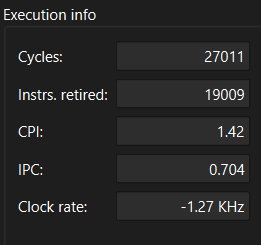
\includegraphics[width=\textwidth]{execinfo2_sin_hazard.png}\\[2pt]
    {\small (a) Sin hazard (con \texttt{nop})}
  \end{minipage}\hfill
  \begin{minipage}[t]{0.42\textwidth}
    \centering
    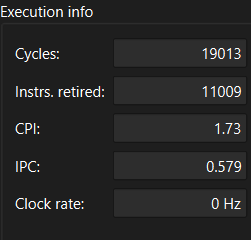
\includegraphics[width=\textwidth]{execinfo2_con_hazard.png}\\[2pt]
    {\small (b) Con hazard (original)}
  \end{minipage}
  \caption{Execution info de Ripes para el programa de saltos. El campo Clock
  rate no se utiliza en el an\'alisis.}
\end{figure}
 
\paragraph{Modelo de ciclos.}
Al modelo de la Parte~1 se le agrega el atasco del \texttt{ecall},
$S_{\text{ecall}}$:
\begin{equation}
  C = N_{\text{instr}} + 4 + 2\,N_{\text{tomados}} + S_{\text{ecall}} ,
  \label{eq:modelo2}
\end{equation}
con $S_{\text{ecall}} = 2$ en el procesador con hazard unit y $0$ en el otro
(secci\'on~\ref{sec:ecall}). Con $N_{\text{tomados}} = 3999$:
\begin{align}
  \text{con hazard:} &\quad 11009 + 4 + 2 \times 3999 + 2 = 19013, \\
  \text{sin hazard:} &\quad 19009 + 4 + 2 \times 3999 + 0 = 27011 ,
\end{align}
que coinciden exactamente con lo medido. Ninguno de los 1001 saltos no tomados
aparece en el modelo.

%----------------------------------------------------------
\subsection{Parte 3: Operaciones entre registros}
%----------------------------------------------------------

\pendiente{c\'odigo final en ensamblador con comentarios que cuantifiquen las
operaciones entre registros (miles), explicaci\'on de por qu\'e funciona,
versi\'on transformada para el procesador sin hazard con su tabla de
dependencias, y resultados de Execution info en los dos procesadores}

%==========================================================
\section{Discusi\'on}
%==========================================================

%----------------------------------------------------------
\subsection{Parte 1: Accesos a memoria}
%----------------------------------------------------------

\paragraph{Los accesos a memoria no cambian.}
Los accesos a la memoria de datos son 4000 en ambos casos: la transformaci\'on
por software agrega instrucciones, pero ninguna toca la memoria de datos. Lo
que s\'i cambia es el tr\'afico de la memoria de instrucciones, que pasa de
14007 a 26007 lecturas como m\'inimo.

\paragraph{El CPI es enga\~noso.}
La versi\'on con \texttt{nop} tiene mejor CPI (1.15 contra 1.29), pero tarda m\'as.
Los \texttt{nop} cuentan como instrucciones retiradas y reducen el promedio sin
hacer trabajo \'util. Contando solo las 14007 instrucciones \'utiles, su CPI
efectivo es
\begin{equation}
  \frac{30013}{14007} \approx 2.14 .
\end{equation}
Por eso la comparaci\'on correcta es en ciclos totales:
\begin{equation}
  \frac{30013}{18013} \approx 1.67 ,
\end{equation}
es decir, el procesador con hazard unit es 1.67 veces m\'as r\'apido con el mismo
programa, y la diferencia es $30013 - 18013 = 12000 = 6 \times 2000$ ciclos,
exactamente un ciclo por cada \texttt{nop} ejecutado.

\paragraph{Hazards de datos contra hazards de control.}
Con forwarding, los hazards de datos de este programa se resuelven sin
atascos: el \'unico sobrecosto que queda son los $2 \times 2001 = 4002$ ciclos de
los saltos, un 22\% del total en el procesador con hazard unit y un 13\% en el
otro. Resolver los hazards de datos por software cuesta $12000$ ciclos, un
40\% del tiempo de la versi\'on con \texttt{nop}. Los hazards de control, en
cambio, no desaparecen con ninguna de las dos soluciones, y requerir\'ian
t\'ecnicas como la predicci\'on de saltos para reducirse
\cite{harris,patterson}.

\paragraph{Limitaci\'on.}
Como el valor cargado por \texttt{lw} no se usa en la instrucci\'on siguiente,
este programa no exhibe el hazard de carga seguida de uso, que ni siquiera el
forwarding resuelve sin un atasco de un ciclo. Un programa que consumiera
de inmediato ese valor mostrar\'ia un costo adicional en el procesador con
hazard unit y m\'as \texttt{nop} en el otro.

%----------------------------------------------------------
\subsection{Parte 2: Saltos}
%----------------------------------------------------------

\paragraph{Solo los saltos tomados cuestan.}
Los ciclos que exceden a las instrucciones son
\begin{equation}
  C - N_{\text{instr}} = 4 + 2 \times 3999 + S_{\text{ecall}},
\end{equation}
sin ning\'un t\'ermino para los 1001 saltos no tomados. Esto confirma que el
pipeline de Ripes contin\'ua buscando instrucciones de forma secuencial mientras
resuelve el salto, lo que equivale a predecir siempre ``no tomado''
\cite{patterson}: cuando acierta, el salto no tiene costo; cuando falla, se
pagan 2 ciclos.
 
\paragraph{Peso de los saltos en el tiempo de ejecuci\'on.}
Los saltos tomados imponen $2 \times 3999 = 7998$ ciclos en ambos
procesadores, un $42\%$ de los 19013 ciclos con hazard unit y un $30\%$ de los
27011 sin ella. Ni el forwarding ni los \texttt{nop} reducen este costo, porque
es un hazard de control y no de datos.
 
\paragraph{El CPI vuelve a ser enga\~noso.}
Igual que en la Parte~1, la versi\'on con \texttt{nop} tiene mejor CPI (1.42
contra 1.73), pero tarda $27011/19013 \approx 1.42$ veces m\'as. La diferencia
de ciclos, $27011 - 19013 = 7998$, corresponde a los 8000 \texttt{nop}
agregados en el ciclo menos los 2 ciclos del atasco del \texttt{ecall}, que
solo ocurre con hazard unit.
 
\paragraph{C\'omo se podr\'ia reducir el costo.}
\begin{itemize}
  \item \textbf{Estructura del ciclo.} Con la condici\'on al final, el ciclo
        necesita una sola instrucci\'on de control por vuelta (\texttt{blt}).
        El programa de la Parte~1, con la condici\'on al inicio, necesita dos
        (\texttt{bge} y \texttt{jal}). Ambas formas pagan un salto tomado por
        vuelta, pero la de la Parte~1 ejecuta una instrucci\'on m\'as por
        vuelta, es decir, 2000 ciclos m\'as en total.
  \item \textbf{Predicci\'on de saltos.} El \texttt{blt} se toma en 1999 de
        2000 ejecuciones, as\'i que un predictor que suponga ``tomado'' para
        los saltos hacia atr\'as acertar\'ia casi siempre. El \texttt{beq}, en
        cambio, alterna entre tomado y no tomado, y un predictor que repite
        el \'ultimo resultado de cada salto fallar\'ia en todas sus
        ejecuciones despu\'es de la primera \cite{smith}.
  \item \textbf{Transformaci\'on de c\'odigo.} Como la paridad de $i$
        alterna, desenrollar el ciclo dos veces (procesar un \'indice par y uno
        impar por vuelta) eliminar\'ia el \texttt{beq} y el \texttt{jal}, es
        decir, al menos 2000 saltos tomados y 4000 ciclos de penalizaci\'on,
        adem\'as de reducir a la mitad las ejecuciones del \texttt{blt}
        \cite{patterson}.
\end{itemize}

%----------------------------------------------------------
\subsection{Parte 3: Operaciones entre registros}
%----------------------------------------------------------

\pendiente{discusi\'on de los resultados de operaciones entre registros y relaci\'on con la teor\'ia}

%----------------------------------------------------------
\subsection{Comparaci\'on de los tres aspectos}
%----------------------------------------------------------

La Tabla~\ref{tab:comparacion} resume los tres programas en los dos
procesadores.

\begin{table}[h]
  \centering
  \begin{tabular}{@{}llrrrr@{}}
    \toprule
    Programa & Procesador & Ciclos & Instrucciones & CPI & IPC \\
    \midrule
    Accesos a memoria & Sin hazard (con \texttt{nop}) & 30013 & 26007 & 1.15 & 0.867 \\
                      & Con hazard                    & 18013 & 14007 & 1.29 & 0.778 \\
    \midrule
    Saltos            & Sin hazard (con \texttt{nop}) & 27011 & 19009 & 1.42 & 0.704 \\
                      & Con hazard                    & 19013 & 11009 & 1.73 & 0.579 \\                 
    \midrule
    Operaciones entre & Sin hazard (con \texttt{nop}) & \pend & \pend & \pend & \pend \\
    registros         & Con hazard                    & \pend & \pend & \pend & \pend \\
    \bottomrule
  \end{tabular}
  \caption{Comparaci\'on de los tres programas en los dos procesadores.}
  \label{tab:comparacion}
\end{table}

\pendiente{discutir la tabla comparativa de los tres aspectos y relacionarla
con la teor\'ia referenciada en IEEE}

%==========================================================
\section{Conclusiones}
%==========================================================

\begin{itemize}
  \item \textbf{Parte 1 (accesos a memoria).} El programa realiza 4000 accesos
        a la memoria de datos (2000 escrituras y 2000 lecturas) en ejecuciones
        de 14007 y 26007 instrucciones, y la memoria queda con los valores
        esperados en ambos procesadores.
  \item La cuantificaci\'on anal\'itica coincide con Ripes: las instrucciones y los
        ciclos reportados se ajustan exactamente al modelo $C = N + 4 + 2N_{\text{saltos}}$.
  \item Resolver los hazards de datos por software mantiene el mismo n\'umero
        de accesos a memoria de datos, pero aumenta las instrucciones un 86\% y
        los ciclos un 67\%, mientras que el forwarding los resuelve sin
        costo en ciclos para este programa.
  \item El CPI por s\'i solo puede ocultar el costo de los \texttt{nop}, por lo
        que la comparaci\'on debe hacerse en ciclos totales.
  \item Los saltos tomados impusieron $4002$ ciclos en ambos procesadores,
        lo que muestra que los hazards de control no los resuelve el forwarding.
  \item \textbf{Parte 2 (saltos).} El programa ejecuta 5000 saltos, de los
        cuales 3999 son tomados y 1001 no tomados, y los contadores confirman
        1000 vueltas por cada camino. Los ciclos medidos se ajustan exactamente
        a $C = N + 4 + 2N_{\text{tomados}} + S_{\text{ecall}}$: solo los saltos
        tomados tienen costo, 2 ciclos cada uno, y representan el 42\% del
        tiempo en el procesador con hazard unit.
  \item El \texttt{ecall} de salida se atiende en EX con hazard unit, con un
        atasco de hasta 2 ciclos, y en ID sin ella, donde puede ejecutarse
        desde el camino equivocado de un salto si \texttt{a7} ya est\'a
        cargado.
  \item \pendiente{conclusiones de la Parte 3 (operaciones entre registros)}
  \item \pendiente{conclusi\'on general que integre los tres aspectos}
\end{itemize}

%==========================================================
\begin{thebibliography}{9}
\bibitem{ripes} M.~B. Petersen, ``Ripes: A Visual Computer Architecture
  Simulator,'' en \emph{2021 ACM/IEEE Workshop on Computer Architecture
  Education (WCAE)}, 2021, pp.~1--8.
\bibitem{harris} S.~L. Harris y D.~Harris, \emph{Digital Design and Computer
  Architecture, RISC-V Edition}. Morgan Kaufmann, 2021.
\bibitem{patterson} D.~A. Patterson y J.~L. Hennessy, \emph{Computer
  Organization and Design RISC-V Edition: The Hardware Software Interface}.
  Morgan Kaufmann, 2017.
\bibitem{smith} J.~E. Smith, ``A study of branch prediction strategies,'' en
  \emph{Proc. 8th Annual Symposium on Computer Architecture (ISCA)}, 1981,
  pp.~135--148.
\bibitem{ripes_src} M.~B. Petersen, ``Ripes: A graphical processor simulator
  and assembly editor for the RISC-V ISA,'' repositorio de GitHub. [En l\'inea].
  Disponible: \url{https://github.com/mortbopet/Ripes}
% \pendiente{agregar mas referencias IEEE sobre pipeline, hazards y jerarquia de memoria}
\end{thebibliography}

\end{document}
